\graphicspath{{12-skeleton/images/}}

\chapter{Various Skeletons}
~\label{c:various_skels}
\greybox{This section contains both literature survey and novel components. As introduced in \emph{Interactive Architectural Modeling with Procedural Extrusions
}\cite{twak11} I contribute both the general intersection event and the mixed weighted straight skeleton. Further contributions are the analysis of the weighted skeleton degeneracies, as ``published'' in a blog post, and the description of the pincushion problem.}


The \emph{straight skeleton} is a geometric subdivision of a 2D shape, based on the notion of ``shrinking'' the shape. In the following we will introduce the skeleton, its properties, degenerate cases, computational complexity, and how to construct it. We extend the standard definition of straight skeleton in several steps, introducing a hierarchy of several skeletons, each of which is a generalisation of the previous. These generalisations introduce additional degeneracies which we catalogue and suggest techniques to resolve. 



Given the spectrum of geometry creation tools explored in Chapter 2, we were searching for an expressive yet simple to use tool that would lie in the centre of our spectrum of proceduralisation. It had to be general enough to create a width range of useful results, but easily controllable without the need for specialist training. As we stumbled upon the idea of offsetting geometry, and were introduced to existing results\cite{Havemann:2005:GMM} relating to the straight skeleton modeling the roofs of buildings, it became clear that the skeleton had the potential of being a powerful modeling tool. The close relation between offsets and the straight skeleton, introduced in Sec.~\ref{sec:ss} formed a powerful argument for this particular geometric primitive having a wide range of modeling applications.

Discovering that the straight skeleton was also heavily used for roofs, we examined how the skeleton could be extended to a larger domain. In the first case we noted that the walls below a skeleton-created roof could be modelled either by an extrusion operation or by the scaling the roof in the vertical direction until it became almost vertical. From this point we explored the generalisation of per-edge slopes in the skeleton. Because the definition of such a structure remained inherently simple and geometric the natural user interface wasn't programmatic, but instead visual.  

In this chapter we examine the straight skeleton in detail and formally introduce a hierarchy of skeletons, each of which takes the same basic information as input, but expresses a wider range of geometric forms than the previous skeleton. In taking this approach we can technical problems underlying the key skeleton concepts of offsetting, or shrinking, a polygon.



% fixme: no correlation with actual work
%We begin by introducing several different ways of shrinking polygons, one in particular has several properties which would make it useful for PGM -- the \emph{straight skeleton}. There are several generalisations of such skeletons; The remainder of the chapter introduces algorithms for their construction, and some of their properties. The edges of these polygons move with constant, positive, negative or arbitrary speeds as the skeleton algorithm shrinks or grows the polygon. With each successive generalisation we introduce new degenerate cases that must be addressed.

%We begin by introducing the straight skeleton, and give one algorithm for its calculation. The following sections review the literature surrounding the skeleton, introducing techniques for reducing the computational complexity, and explaining some of its mathematical properties. We explore some of the degenerate conditions that can occur when constructing the skeleton and introduce our \emph{general intersection event} to overcome a several of these. Finally we introduce two variants of the straight skeleton, and discuss their degenerate cases. 

\section{Ways of Shrinking Polygons}
\label{sec_ways_of_shrinking}
There are many ways in which to shrink a polygon. Fig.~\ref{fig:offset_types} illustrates four published techniques which translate shrinking edges in a self-parallel manner. These techniques only vary in their treatment of reflex corners:
\begin{enumerate}[a)]
%\setcounter{enumi}{1}
\item  Given that each edge moves towards the inside of the polygon (green), parallel to itself (white arrows), a multitude of techniques can be imagined by changing the handling of the corners.
\item The \emph{medial axis}~\cite{Blum67}. A reflex vertex becomes a parabola as it shrinks, maintaining a constant distance from the original polygon. The medial axis itself is a skeleton defined as the set of all points within the polygon which are equidistant to two or more points on the boundary of the polygon.
\item The straight skeleton\cite{Aichholzer95} (SS), moves reflex verticies with the intersection of the two adjacent edges. We investigate further properties of the straight skeleton in Sec.~\ref{sec:ss}.
\item The \emph{linear axis}~\cite{Tuanase:2004} introduces \emph{hidden edges} into reflex corners of the skeleton to approximate the medial axis using only straight line segments. These hidden edges immediately grow to ``blunt'' such verticies, reducing their ``speed'' as the polygon shrinks.
\item A weighted variation of the straight skeleton (\emph{WSS}) was introduced by similarly timed later papers by both Eppstein and Erickson~\cite{Epp:98}, as well as Aicholzer and Aurenhammer~\cite{Aichholzer:1996:SKF}. Both papers only give a passing mention to WSS and degenerate cases are not introduced. The edges of the WSS are assigned independent speeds for shrinking, which shall be examined further in Sec.~\ref{s:pwss}.
\end{enumerate}

\begin{figure}[htb]
  \centering
  \def\svgwidth{1.\columnwidth}
  \includesvg{12-skeleton/images/offset_types}
  \caption[Different ways to shrink a polygon.]{\label{fig:offset_types}Techniques to shrink a polygon (a). These include the medial axis (b), straight skeleton (c), linear axis (d) and weighted straight skeleton (e). The result of using each technique to shrink the polygon by a small distance is shown (the light green areas are lost to the shrinking process).}
\end{figure}

Our interest here is in the straight skeletons (SS and WSS), as these structures do not introduce curved or additional edges, and, as demonstrated in Chapters~\ref{c:pgop} and \ref{c:procex}, are well suited to modeling certain classes of man-made objects as 3D meshes.

\section{The Straight Skeleton}
\label{sec:ss}

\begin{figure}
  \centering
  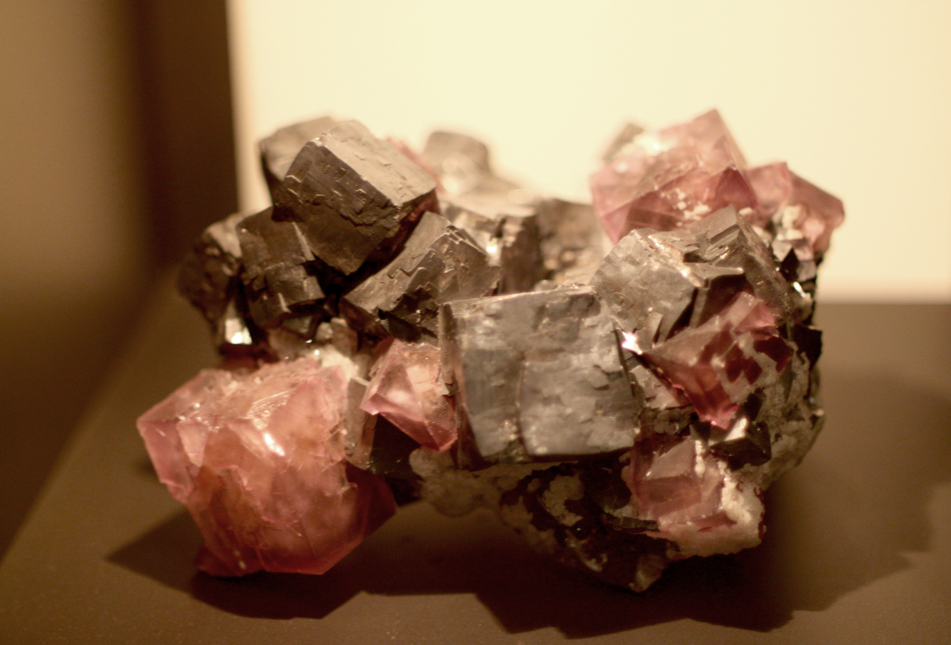
\includegraphics[width=1.0\columnwidth]{crystal.png}
  \caption[Purple cubic crystals of fluorite]{\label{fig:crystal}Composite grey cubit crystals of galena with purple cubic crystals of fluorite. Cave-in-rock, Hardin Co., Illinois, USA.}
\end{figure}

Let us consider the growth of a crystal, as in Fig.~\ref{fig:crystal}. As Aichholzer observed in \cite{Aichholzer:1996:SKF}, if we were to watch such a crystal growing we would see that each face grows outwards in a self-parallel manner, and the edge between two such faces moves outwards as the intersection of these faces. Thijssen et al.\cite{Thijssen92} earlier explored the statistical properties of such growth in crystals, introducing a 2D proxy for the original 3D geometry, Fig.~\ref{fig:skel_crystal}. This model of self-parallel growth is the reverse of the process that is performed to calculate the straight skeleton, which is calculated by the shrinking of a polygon.

\begin{figure}
  \centering
  \def\svgwidth{1.\columnwidth}
  \includesvg{12-skeleton/images/crystal}
  \caption[2D crystal growth.]{\label{fig:skel_crystal} Given a set of square seeds (grey) on a line, the polycrystalline growth moves outwards (green), and the movement of the corners traces out lines (blue).}
\end{figure}

The straight skeleton (SS) is a 2d graph of \emph{arcs} generated from this shrinking of a polygon. Each of the edges of the polygon moves towards the interior at a constant speed in a self-parallel manner. Occasionally the topology of the polygon changes as we observe \emph{events} such as an edge shrinking to zero length. As shown in Fig.~\ref{fig:skel_shrink}, the movement of the corners of the decaying polygon trace out the ``skeleton'' itself. These arcs describe the path of the verticies as the polygon shrinks. Several examples are shown in Fig.~\ref{fig:skel_examples}.

\begin{figure}
  \centering
  \def\svgwidth{0.7\columnwidth}
  \includesvg{12-skeleton/images/skel_shrink}
  \caption[Shrinking a polygon to form the straight skeleton]{\label{fig:skel_shrink}Left: A shrinking polygon. Right: The arcs of the straight skeleton (blue) are formed by tracing the edges of the shrinking polygon.}
\end{figure}


\begin{figure}
  \centering
  \def\svgwidth{1.0\columnwidth}
  \includesvg{12-skeleton/images/skel_examples}
  \caption[The straight skeleton of various polygons]{\label{fig:skel_examples}A variety of polygons (green) and their straight skeletons (blue).}
\end{figure}


\subsection{Constructing the Straight Skeleton}
\label{sec:constring_skeletons}

The SS is a graph of straight edges in $\mathbb{R}^2$. However we can interpret it as a \emph{terrain} -- a set of faces in $\mathbb{R}^3$ which form a ``landscape''\cite{Aichholzer95}, Fig.~\ref{fig:skel_terms} right. This approach is taken as it allows a comparison between the standard, unweighted straight skeleton, and the various types of weighted straight skeletons (WSS), a generalisation introduced in Sec.~\ref{s:pwss}.
The terrain constructed touches the polygon on each edge, and the projection of the edges of the terrain onto the polygon forms the 2D straight skeleton. 

The shrinking process is modeled as a sweep plane that rises with constant speed from the input polygon, carrying with it the evolving shape. Each edge of the polygon moves inwards with a constant speed relative to the sweep plane motion. The sweep plane rises and the polygon shrinks, encountering various topological events. Eventually the polygon shrinks to nothing and the skeleton is complete. The terrain approach allows the events to be modelled as the intersection of three planes, rather than three 2D edges, allowing the geometry of Chapter~\ref{c:procex} to be constructed trivially.

\begin{figure}[hb]
  \centering
  \def\svgwidth{1.0\columnwidth}
  \includesvg{12-skeleton/images/skel_terms}
  \caption[Straight skeleton terminology]{\label{fig:skel_terms}Straight skeleton terminology. The input plan defines the starting state of the construction, while the active plan defines the state part way through the shrinking process. The final straight skeleton is a 2D graph consisting of arcs adjacent to faces. The roof model is an alternative 3D representation, the projection of which onto the ground plane forms the 2D straight skeleton.}
\end{figure}

To distinguish between the under constrained term ``polygon'' and a similar structure with additional constraints, we introduce a \emph{plan}, Fig.~\ref{fig:skel_terms}. A plan is a  planar partition (a straight line planar embedding of a planar graph) that divides the plane into finite \emph{inside} and infinite \emph{outside} regions. 
A plan is a set of polygons consisting of corners and edges, these are embedded in a plane parallel to the $xy$ (``ground'') plane, so that all corners of a plan have the same $z$ (height) value. The $j$th polygon is described by $n^j$ polygon corners $c^j_i \in \mathbb{R}^3$ with $1 \leq i \leq n^j$.  Each corner $c^j_i$ is connected to the next corner (according to the polygon orientation) by an \emph{edge} $e^j_i$. 
The loops of edges are oriented counter-clockwise, but polygons describing holes are oriented clockwise. 
Additional bounded regions may be recursively located inside a hole. 
When discussing plans, indices are treated cyclically, so that in a polygon with corners $c^j_1$, $c^j_2$, and $c^j_3$, the vertex $c^j_4$ means $c^j_1$.

Unlike the medial axis, there is no trivial description as to whether a particular point within a polygon lies on the SS arcs. Instead, the skeleton is defined in the literature as the result of the process of shrinking a polygon. That is, the only description of the SS we have, is the algorithm for its construction.

To construct the skeleton, a sweep plane rises vertically from the \emph{input plan}. This sweep plane carries with it an \emph{active plan} that defines cross sections of the terrain. This 3D approach was first suggested by Eppstein et al.~\cite{Epp:98}, although in spirit similar to the original 2D proposal by Aichholzer\cite{Aichholzer95}, with data structures inspired by Felkel and Obdr\v{z}{\'a}lek\cite{Felkel98}. However we use our own notation for continuity. The output of the system is a series of \emph{skeleton faces} that make up the 3D terrain. The edges between the faces are named \emph{arcs} after Aichholzer et al.\cite{Aichholzer95}, a term that we shall use in both 2D and 3D interpretations of the skeleton.
%The projection of the arcs onto the plane of the input plan is the 2D SS as in Fig.~\ref{fig:skel_terms} right. 

As the SS is constructed, the sweep plane rises with constant speed, and the active plan shrinks. In the case of the basic straight skeleton every plan edge moves with a constant and uniform speed towards the interior of the polygon. As both the speed of the sweep plane and plane edges are constant, each plan edge remains within the same 3D plane. One of these \emph{direction planes} is associated with, and intersects, every edge in the input plan. As both the speed with which the sweep plane rises and the movement of the edges is equal, the direction plane associated with each edge  $e^j_i$ forms an angle $\pi/4$ with the input plane. Each skeleton face lies in one of these direction planes. To obtain a steeper or shallower roof from the SS we may scale the faces in the $Z$ direction appropriately. 

At all times in this shrinking process we must ensure that the active plan remains \emph{well formed}. That is:

\begin{itemize}
\item{The enclosed region remains to the left of every directed edge.}
\item{No edge intersects another edge, with the exception of touching the neighbouring edges only at shared corners.}
\item{Every enclosed region has a positive, finite and non-zero area.}
\item{There must be a finite number (zero or more) of such enclosed regions.}
%\item{No overlapping edges exist.}
\end{itemize}

%(edges intersect adjacent edges at their endpoints) 
In the SS every active plan edge has the same constant, positive, speed. As the edges move, the corners remain defined by the intersection of the adjacent direction planes and the current sweep plane, as in the plans of Fig.~\ref{fig:skel_edge}. Therefore each corner in the active plan, $c^j_i$, moves between events with a constant, and often unique, speed and slope relative to the input plan.

\begin{figure}
  \centering
  \def\svgwidth{0.8\columnwidth}
  \includesvg{12-skeleton/images/skel_edges}
  \caption[A moving plan edge]{\label{fig:skel_edge}As the active plan shrinks, the edges move with a constant speed. Several plans (left, middle, right) are shown (green), along with their shape at a later time (grey lines). In a certain time, every edge moves the same distance ($x$), but movement of the corners is defined as the intersection of the corners and so the distance moved typically varies. Very sharp reflex or acute angles between edges may cause corners to move with high speed (right). This speed approaches infinite as the interior angle approaches $2\pi$ from below, or $0$ from above.}
\end{figure}

Fig.~\ref{fig:skel_inverted} shows that as sweep plane rises and the active plan shrinks, the plan may become badly formed (red). To ensure that the active plan remains well formed, we detect when more than two or more edges intersect and we make topological changes to the active plan.  We call these \emph{events}; as introduced by Aicholzer et al.~\cite{Aichholzer95} there are two types of event:

\begin{figure}
  \centering
  \def\svgwidth{1.0\columnwidth}
  \includesvg{12-skeleton/images/skel_inverted}
  \caption[A badly formed plan]{\label{fig:skel_inverted} Left: the anti-clockwise oriented input plan. Middle: The active plan at a split event (orange). Right: Without a split event, a portion of the active plan becomes badly formed. There are self-intersections at a and b, and the red region is defined by a clockwise loop; that is, the edges define an infinite inside region outside the red area.}
\end{figure}

\begin{itemize}
\item
\emph{Edge events} occur as the length of an edge shrinks to zero. When a plan edge shrinks to zero the direction planes defined by three consecutive (linked by corners) edges collide (Fig.~\ref{fig:skel_intro}, 2). 
\item
\emph{Split events} take place when two adjacent direction planes, and one non adjacent direction plane collide (Fig.~\ref{fig:skel_intro}, 3). These split the region bounded by the active plan into two parts. 
\end{itemize}.

\begin{figure}
  \centering
  \def\svgwidth{1.0\columnwidth}
  \includesvg{12-skeleton/images/skel_intro}
  \caption[Constructing the straight skeleton]{\label{fig:skel_intro} Left: the straight skeleton is given by arcs (blue lines) tracing the verticies of a shrinking polygon (black lines). Each edge moves with a constant speed towards the interior of the polygon, and as it does the topology of the polygon changes in several different ways (dark green lines), during \emph{events}. Right 1-3: The calculation of the SS is primarily a sequence of such events. 
%Right 4: We can view the skeleton as a 3d structure with polygonal faces. The final skeleton, without the intermediate shrinking stages is shown at the bottom of the figure.
}
\end{figure}


\begin{figure}
  \centering
  \def\svgwidth{1.0\columnwidth}
  \includesvg{12-skeleton/images/skel_unweighted_intro}
  \caption[Split and edge events]{\label{fig:skel_unweighted_intro} Edge (a) and split (b) events that occur as a polygon shrinks. Peaks (c \& d) comprise three co-sited edge events.}
\end{figure}

%After an event, the well-formed property must hold for the plan in two circumstances:
%\begin{itemize}
%\item{The plan must remain well formed globally. There are situations in which just being well-formed locally is not sufficient.}
%\item{As the edges involved in the event continue to move across the active plan immediately after the event, they may not become badly formed. However, a new edge not involved in the original collision may form a second event. This is made easier by the sector property introduced later.}
%\end{itemize}

We can describe these events in terms of the local plan around the direction plane intersection point, Fig.~\ref{fig:skel_unweighted_intro}. Here we see the local active plan region before, during and after edge events (a), split events (b) as well as peaks (c \& d). As these peaks may be considered to be three edge events occurring together, we classify them as edge events.

Each of these events is witnessed by the intersection of three direction planes. However not all intersections between three unbounded direction planes indicate an event. As identified in Fig.~\ref{fig:skel_intersecting_planes}, we must be sure that the faces intersect within the bounds of the associated edges on the active plan. Also of interest to optimisation is that at least one pair of adjacent plan-edges must be involved; an SS event consists of three edges, at least two of which must be adjacent.

\begin{figure}
  \centering
  \def\svgwidth{0.85\columnwidth}
  \includesvg{12-skeleton/images/skel_planes}
  \caption[Not all direction plane intersection are active plane events]{\label{fig:skel_intersecting_planes}The active plan in two configurations in which intersection of unbounded direction planes (intersection with active plan shown as red, cyan and orange lines) does not lead to an event as they occur outside the bounds of the associated edges.}
\end{figure}

Every event creates one or more output arcs, a portion of the boundary of a terrain face. Every arc is the boundary between two faces.

We present a crude algorithm in Fig.~\ref{code:skelcode} that maintains this queue as new corners are introduced by events. We defer describing the event handling in detail until Sec.~\ref{s:gie}, noting that Felkel~\cite{Felkel98} simply gives a terse set of manipulations to the data structure in the case of edge or split events.

The active plan is stored in a data structure that holds the corners of each polygon in a doubly linked list, as illustrated in Fig.~\ref{fig:skel_datas_structures}. There is such a list for every polygon and associated holes. Each corner, therefore, has a pointer to its next and previous corners (assuming counterclockwise order), as well as a pointer to its previous and next direction planes. The corner is a point in $\mathbb{R}^3$ at the lowest intersection of the adjacent plan edges. We may find the position of a corner in the active plan by intersecting the corner's next and previous direction planes with the sweep plane. Correspondingly, an edge on the active plan is given by the positions of two consecutive corners in the linked list. In this manner the linked list implicitly stores the active plan at the sweep plane, via corners at or below the plane. 
% todo: illustration of linked list implicitely storing a polygon at the sweep plane.
\begin{figure}
  \centering
  \def\svgwidth{1.0\columnwidth}
  \includesvg{12-skeleton/images/skel_data_structures}
  \caption[The implicit active plan]{\label{fig:skel_datas_structures}Left: The initial set of corners (yellow circles) and points in the doubly linked list (yellow arrows) that make up the input plan. Not shown are the pointers to the adjacent direction planes. Centre: As the sweep plane rises, and various events occur the active plan may split. Corners are added and removed from the linked lists. Here two linked lists store an active plan with two polygons (yellow, purple lists). Right: By projecting the intersection of the corner's direction planes onto the sweep plan, we store the implicit active plan (purple, yellow polygons)  }
\end{figure}

To simulate the rising sweep plane approaching events, a priority queue ordered by height ($z$) is kept, specifying triplets of edges colliding at a certain height. We assume that the queue only holds one event for each unique set of colliding direction planes.
Before an event is processed, the algorithm checks that it is at or above the sweep plane, and within the current bounds of each face --- previous edge events may even have removed the edges and their direction planes entirely.
The details of the \emph{HandleEvent} routine of Fig.~\ref{code:skelcode} are introduced in the following section, which may add arcs to faces, and add or remove corners and edges from the active plan.  Arcs are stored in a list associated with each input-edge; events add arcs to these lists. The algorithm continues until all events in the queue have been processed. After all events have been processed we traverse an input-edge's arcs in a counter clockwise direction to determine the 3D face. This process is illustrated in Fig~\ref{fig:skel_reconstruct_faces}.

\begin{figure}
  \centering
  \def\svgwidth{1.0\columnwidth}
  \includesvg{12-skeleton/images/skel_reconstruct_faces}
  \caption[Reconstructing skeleton faces]{\label{fig:skel_reconstruct_faces}Left: After all events have been processed, every arc is associated with two input plan edges. Middle: A single input plan edge has a set of edges, which may be traversed (right) in a counter clockwise direction to construct a face (right, orange).}
\end{figure}


\begin{algorithm} [htb]
\begin{footnotesize}
  Main \Begin{
   $Q$ = new priority queue\; 
   $sweepZ$ = 0\;

    \ForEach{ corner $c$ in active plan } {
        CreateGIEEvents ( $c$, $Q$ )\;
    }

    \While { !$Q$.empty() } {
        event = FindNextEvent($Q$)\;%sWithin( $\delta_2$ )\;

        event.removePlanesNotInActiveplan()\;
        event.removePlanesOutOfBounds()\;
	\If { event.getPlanes().size() $\ge$ 3) and \newline
              event.z $\ge$ $sweepZ$ } 
              %event.withinBounds() }%and\
              %!seenTriples.contains(event.p1, event.p2, event.p3) }
        {
            $newCorners$ = HandleEvent( event )\;
            
            $sweepZ$ = event.$z$\;
%            $seenTriples$.add(event.p1, event.p2, event.p3 )\;
            \ForEach{ corner $c$ in newCorners }{
              CreateEvents($c$, $Q$)\;
            }
        }
    }

    \ForEach{ edge $e$ in input plan } {
         ReconstructFace ($e$)\;
    }
}

  CreateGIEEvents( corner $c$, queue $Q$ ) \Begin{
     $p1$ = $c$.nextEdge.getPlane()\;
     $p2$ = $c$.prevEdge.getPlane()\;
     \ForEach{ direction-plane $p3$ in the input} {
 %       \If {!seenTriples.contains ($p1$,$p2$,$p3$)} {
        $location$ = Intersect ($p1$, $p2$, $p3$)\;
        $Q$.insert (new Event($location$, $p1$, $p2$, $p3$))\;
 %          } 
     }
   }
\end{footnotesize}
  \caption{Pseudo-code for the SS algorithm}
  \label{code:skelcode}
\end{algorithm}


Given a ``random'' or irregular input plan these two (split and edge) event types are the only features we are likely to see, Fig.~\ref{fig:wss_complex_three_event}. This is because the skeleton of irregular polygons rarely have events where more than 3 faces meet at one point. 

\begin{figure}
  \centering
  \def\svgwidth{0.85\columnwidth}
  \includesvg{12-skeleton/images/wss_complex_three_event}
  \caption[A complex straight skeleton]{\label{fig:wss_complex_three_event} The straight skeleton of a complex plan in which only three faces meet at every node in the graph.}
\end{figure}

%todo:
%abstract a ``resolve event'' stage.
%introduce queues and ray-casting to identify split events.
%after event, re-cast.

\FloatBarrier

\subsection{Computational Complexity of the Straight Skeleton}

%introduce triangulation, motorcycle graph etc...
% introduce the fact that reflex verticies cause most of the trouble.

%todo is the ocmplexity for our algorithm correct.
%todo verify complexities here
%todo, city huber's thesis

The algorithm presented in the previous section, Fig.~\ref{code:skelcode}, runs in a time complexity of $O(n^2 \log n)$, where the number of input plan corners is $n$. This is due to the observation that there are a maximum of $n$ events that must each search for new adjacent planes to intersect ($O(n^2)$), and insert any new events into the priority queue ($\log n$). Filling the priority queue initially also takes $O(n^2 \log n)$ time.

Originally Aichholzer et al.  presented a similar analysis in 2D\cite{Aichholzer95},  and a variation with a similar result\cite{Aichholzer95:SSSP}. These papers also prove the above lemma stating the number of events is $O(n)$. It is also given that calculating the SS of a convex polygon is possible in $O(n \log n)$ time since an edge on the active plan will only intersect with its neighbours. The higher complexity in the concave case is caused by the propagation of reflex verticies, and the requirement to identify which other edge they intersect with. 

The following year Aichholzer and Aurenhammer\cite{Aichholzer:1996:SKF} introduced an elegant method that triangulates the active plan.%The the simulation of a collapsing triangulation of the active plan. 
The key observation is that every event is witnessed by a shrinking triangle reaching zero area and collapsing, Fig~\ref{fig:skel_triangulation}. By keeping a list of triangles, ordered by their collapse time, the propagation of the offset (wavefront) is simulated. This would give a linear time complexity, except that the collapse of certain triangles does not signify an event. Due to an inability to place a non-trivial bound on these \emph{flip} events, the algorithm has a total time complexity of $O(n^3 \log n)$. Recent research has lead to strong evidence that such an algorithm delivers $O(n)$ performance in practice\cite{Palfrader12}. 
%todo: 2.6 summary in huber's thesis states worst case is $O(n^3 log n)$. (or only implmentable?)

\begin{figure}
  \centering
  \def\svgwidth{0.85\columnwidth}
  \includesvg{12-skeleton/images/skel_triangulation}
  \caption[Aicholzer's triangulation algorithm]{\label{fig:skel_triangulation}Aicholzer introduced a triangulation based algorithm\cite{Aichholzer:1996:SKF} for the calculation the Straight Skeleton in 1996. As the shape shrinks, the events (above; left to right) are each witnessed by a collapsing triangle in the triangulation (bordered by white lines). By ordering the triangles by their collapse time, it is possible to identify a correct sequence of events.}
\end{figure}

Eppstein and Erickson\cite{Epp:98} introduced the sweep-plane component used in the previous algorithm to construct a 3D terrain. This was augmented by a powerful closest-pairs data structure and advanced ray-casting techniques to give a sub-quadratic time complexity of $O (
n^{1+\epsilon} + n ^{8/11+\epsilon} r ^{9/11 + \epsilon})$, where r is the number of reflex verticies, and $\epsilon$ is a arbitrarily small constant controlling time/space trade off. Given that $r$ is of order $O(n)$, and as $\epsilon$ approaches $0$, a time complexity of $O(n^{17/11})$ is achieved.

Eppstein and Erickson also introduced a model of the problematic reflex verticies - that of calculating the \emph{motorcycle graph}. A brief introduction is given in Fig.~\ref{fig:skel_motorcycle}. Chen and Vigneron\cite{Cheng02} continued this work to produce an algorithm that isolates parts of the skeleton based on the motorcycle graph. Chen's algorithm to calculate the motorcycle graph in a time of $O(r\sqrt{r}\log r)$ leads to a randomised algorithm to calculate the skeleton with a lower bound of $O(n \log^2 n + r\sqrt{r}\log r)$.

\begin{figure}
  \centering
  \def\svgwidth{0.85\columnwidth}
  \includesvg{12-skeleton/images/skel_motorcycle}
  \caption[Eppstein's Motorcycle Graphs]{\label{fig:skel_motorcycle}Eppstein's motorcycle\cite{Epp:98} graph divides the polygon (left) into concave regions, considering only the reflex verticies (orange points) and their propagation (orange line) with time. These propagation lines may not be crossed by another vertex, if they do the vertex terminates (red points). The time complexity of constructing such a graph is introduced as $O(n^{3/2})$. The resulting tessellation of the polygon may then be used as an acceleration structure when constructing the straight skeleton.}
\end{figure}

Recently Huber et al. introduced a robust, implementation-oriented approach with time complexity $O(n^2 \log n)$, which exhibited $O(n \log n)$ in practice. The algorithm introduces additional Steiner verticies to account for the effects of reflex verticies.

\begin{comment}
\subsection{Properties of the Straight Skeleton}

%todo:
\begin{itemize}
\item Raindrop property\cite{Aichholzer95}.
\item The faces of the resulting skeleton are monotone in a direction perpendicular to their associated input-plan edge\cite{Aichholzer:1996:SKF}. This is a consequence of every edge in the active plan moving with the same speed.
\item As we may guess from the complexity results, and our earlier comments on corner speed, reflex verticies are significant as they may move with high speed. Fig.~\ref{skel_examples} row 2, columns 1-3 give examples of situations in which the exact positioning of reflex verticies play a significant part in the final shape of the skeleton. We may describe the skeleton in these situations as highly chaotic; small changes in the input polygon cause large changes in the output.
\item Rotational invariance. Good for shape descriptors. Linear axis cite.
\end{itemize}

%Several other interesting features of the SS have been noted in the literature.
%\begin{itemize}
%\item unable to define globally like medial axis (), so is a procedural procedural primitive
%\item water-drop property
%\item monotonicity of hte faces
%\item eppstein's slabs
%\item chaotic: small changes lead to big outcome differences
%\end{itemize}
%\quote{Unlike the Voronoi diagram of G, the straight skeleton of G has no meaningful interpretation in the distance model}\cite{Aichholzer:1996:SKF}
\end{comment}

\subsection{Straight Skeleton Degenerate Events}
\label{s:ssd}

Thus the algorithm presented in Sec.~\ref{sec:constring_skeletons}, in line with the literature, is applicable to general input plans, however in contrived \emph{degenerate} situations, we may see complex arrangements of active plan edges intersecting at a point. The previous work leaves these events badly defined; here we detail several observed situations: \emph{loops of two}, \emph{many edges colliding} and \emph{parallel consecutive edges}. In contrast, the following Sec. \ref{s:gie} will introduce a \emph{general intersection event} which calculates a well-formed active plan after all events -- edge and split events, as well as the degenerate cases introduced here.

The literature is limited in its discussion of events. The original work by Aichholzer\cite{Aichholzer95} describes split and edge events, but does not describe an algorithm to compute them. Eppstein\cite{Epp:98} presents the \emph{many edges colliding} degeneracy, under the classification \emph{vertex events}, but does not detail an algorithm to resolve them. Only the work by Felkel\cite{Felkel98} explicitly addresses the topology manipulation at events, but then does not discuss degenerate events, beyond a special check for \emph{loops of two}. As we introduce generalisations of the straight skeleton, these degenerate events and the algorithms used to resolve them become more important.

Fig~\ref{fig:skel_unweighted_intro_2}, c,d and e, shows one degenerate case in which the active plan becomes a region with only two edges and zero area, a \emph{loop of two} degeneracy. A more involved example is shown in~\ref{fig:skel_loop_two}. After all the events at a certain height, parallel edges may cause the active plan to become partially or entirely composed of these zero-area regions. Felkel at al.\cite{Felkel:1998:SKI} require a special case to identify and remove these degeneracies. 

\begin{figure}
  \centering
  \def\svgwidth{1.0\columnwidth}
  \includesvg{12-skeleton/images/skel_unweighted_intro_2}
  \caption[Various degenerate situations]{\label{fig:skel_unweighted_intro_2} In degenerate situations, more than three edges will collapse at one time (a,b \& e). We also note that sometimes the active plan collapses to a \emph{loop of two} (c,d \& e). We show these coincident edges as curved lines, with asterisks.}
\end{figure}

\begin{figure}
  \centering
  \def\svgwidth{1.0\columnwidth}
  \includesvg{12-skeleton/images/skel_loop_two}
  \caption[An example of the loop of two situation]{\label{fig:skel_loop_two} A more complex example of a straight skeleton, left, that creates a zero area plan, right. Note that the curved line segments are in reality straight, but again drawn as curved segments to represent the topology.}
\end{figure}

Another type of degeneracy occurs as four or more plan edges collide at a point, the \emph{many edge degeneracy}. Several connected edges may intersect at the same time, as illustrated in Fig~\ref{fig:skel_unweighted_intro_2} a, in which only the first and last edges exist after the event, as the intermediate edges shrink to zero length. 
Alternatively we may see reflex verticies in the input plan form several connected sets of edges involved in a single event, as in Fig~\ref{fig:skel_unweighted_intro_2}, b.  These types of events are ignored in some of the earlier work\cite{Aichholzer95}, introduced as a third type of \emph{vertex} event in \cite{Epp:98}, and dramatically changes the expected time complexity of the algorithm in \cite{Cheng02}.

A final degenerate case occurs when adjacent, yet parallel, edges in the active plan become consecutive, the \emph{parallel consecutive edge} (PCE) degeneracy.
Fig.~\ref{fig:skel_linear_ambig} demonstrates such a case. Because we have defined the movement of corners over the active plan, the intersection of the adjacent direction planes, the intersection of parallel collinear edges neighbouring a corner is a line, rather than point, causing a special case to arise. Existing work\cite{Aichholzer95} leaves the outcome undefined. It appears that there are two resolutions techniques applicable to this degeneracy:
\begin{itemize}
\item The \emph{separate} solution shown in Fig.~\ref{fig:skel_linear_ambig}, left-centre.  After the PCE, the faces remain separated by an arc. This approach maintains a single face for every edge in the input plan. However defining the movement of such a vertex is problematic as the adjacent direction planes are coincident. 
\item The \emph{merge} solution illustrated in Fig.~\ref{fig:skel_linear_ambig}, right-centre. When a PCE occurs, the two faces are joined together. This has the advantage that no vertex is created with parallel adjacent edges. However this removes the one-to-one mapping between the edges in the input plan and the output skeleton faces.
\end{itemize}
In the unweighted case a further resolution is to define a special case for this situation. In this case the corner would move perpendicularly to both the neighbouring plan edges, towards the interior of the plan. This is inelegant, and is not able to generalise to the weighted case in Sec.~\ref{s:pwss}.

\begin{figure}
  \centering
  \def\svgwidth{1.0\columnwidth}
  \includesvg{12-skeleton/images/skel_linear_ambig}
  \caption[An issue with parallel consecutive edges]{\label{fig:skel_linear_ambig} Left: The PCE problem: What is the resolution to the event marked a? Left-Centre: The separate rule. Right-Centre: the merge rule. Right: When there are PCE in the active plan, a resolution must still be applied to determine the initial direction and speed of the corner.}
\end{figure}

It is interesting to note that~\cite{Aichholzer95} seems to exclude such PCE in the input, however there is no easy way to tell if parallel edges will become consecutive as the skeleton is constructed. By symmetry we would expect to see PCEs in the input computed using the same solution, as illustrated in Fig.~\ref{fig:skel_linear_ambig}, right.

The PCE resolution technique chosen in a given SS implementation will depend on the desired properties of the resulting skeleton.

In order to process any of these degenerate events it may be suggested that we perturb the active plan slightly. However, as in Fig.~\ref{fig:skel_reflex_combine} from  Eppstein and Erickson\cite{Epp:98}, there are situations in which small perturbations cause undesirable large changes in the resulting skeleton. In this situation two input reflex corners form a third reflex corner during evaluation. It is therefore necessary for a single event to process collisions between many direction planes. The earlier Fig.\ref{fig:skel_examples}, bottom right, gives another example where successive pairs of reflex corners meet, are resolved, and carry on to create additional reflex corners.

\begin{figure}
  \centering
  \def\svgwidth{0.6\columnwidth}
  \includesvg{12-skeleton/images/skel_reflex_combine}
  \caption[Perturbing event sequences may lead to wildly different results]{\label{fig:skel_reflex_combine}Figure from~\cite{Epp:98}, demonstrating that perturbing the sequence of events at a point (orange), rather than solving them together, may lead to wildly different results (left).}
\end{figure}

\FloatBarrier
\subsection{The Generalised Intersection Event}
\label{s:gie}

This section demonstrates that we can unify the split, edge and vertex events into a \emph{generalised intersection event} (GIE). This avoids the involved categorisation in the literature and allows a single algorithm to compute well formed results, even when events contain loop of two, PCE or many edge degeneracies.
%There is no particular reason that these events must be solved in this manner - many other ways to ensure the plan remains well formed can be imagined - however

The GIE is consistent with the split and edge events observed on the active plan.

We begin by defining \emph{chains} of edges that are involved in an event, Fig.~\ref{fig:skel_chains}. A chain is a list of consecutive edges that are colliding at the event. They are ordered corresponding to the edge's direction. These form the partial boundary to our possibly bounded topological disc region of the active plan that is collapsing at the event.

\begin{figure}
  \centering
  \def\svgwidth{0.5\columnwidth}
  \includesvg{12-skeleton/images/skel_chains}
  \caption[Adjacent edges in an event form chains]{\label{fig:skel_chains} Two regions of active plans corresponding to Fig.~\ref{fig:skel_unweighted_intro_2}b on the left and Fig.~\ref{fig:skel_unweighted_intro_2}a on the right. We can group the active plan edges involved in an event into chains (red, yellow and blue edges) by asking which edges are consecutive in the linked list data structure.}
\end{figure}

In the case of the SS we can order the chains themselves around the event's location, Fig.~\ref{fig:skel_gie_intro} d. That is the chains themselves may be ordered in a cyclic list. %Immediately before the event the location of the event is always within the region bounded by the active plan.
We can note that after an event the last edge in the preceding chain, and the first edge in the following chain become adjacent, Fig.~\ref{fig:skel_gie_intro} c and e.

\begin{figure}
  \centering
  \def\svgwidth{0.8\columnwidth}
  \includesvg{12-skeleton/images/skel_gie_intro}
  \caption[Chains approaching an event]{\label{fig:skel_gie_intro} As three chains approach an event (a, orange), we can imagine the active plan at the event (b), or the degenerate plan if no event takes place (c). We observe that the last edge in the previous chain and the first edge in the following chain become adjacent, also that every chain is split into two (f). Given that the angles between adjacent chains (d, $\alpha$, $\beta$ \& $\gamma$) may not overlap and that all edges are moving towards the interior, the directions of the new inter-chain verticies (e, $A$, $B$ \& $\Gamma$) are unique and non-intersecting. Hence the new topology (f) does not self-intersect.}
\end{figure}

The intuition behind the GIE is that at an event's location, an inside area on the active plan collapses and transitions to an outside area. As this occurs, adjacent chains that before bounded interior regions split in two, with the two halves of adjacent chains now bounding an exterior region. These newly created chains do not intersect each other as their single shared vertex is moving away from the event's location, in a unique direction. This direction is bounded by the two edges of the new chains, as in Fig.~\ref{fig:skel_gie_intro} d, and ensures a solution free of self-intersections. Therefore, our algorithm first removes edges that shrink to zero length, and then ``cycles'' the chains in such a manner to bound the interior regions.

To resolve an event using the GIE we firstly pre-process the edges involved in the clustered intersection events into a set of \emph{chains}. A chain defines a connected portion of the active plan boundary involved in the event. A chain, $h^i$, is a list of consecutive active plan edges, $\epsilon^i_1...\epsilon^i_{hmax_i}$. A cyclic \emph{chain list}, $b$, contains all such chains, $h^1...h^{bmax}$ (we assume a cyclic index). The chain list is ordered by the edge's orientation around the intersection. After this pre-processing we perform the following sequence of steps, a pseudocode summary is given in Fig.~\ref{code:gie_pseudocode}. 

\begin{itemize}
\item{\emph{Intra chain step} (Fig.~\ref{fig:skel_intra}): Within each chain, any edges in the middle (not the first or the last edge in a chain) shrink to 0-length and are removed from the active plan. Formally, we remove all interior edges from a chain $h^i$, leaving only the start, $\epsilon^i_1$, and the end, $\epsilon^i_{hmax_i}$,  of the chain. That is, if $hmax_i \ge 3$, then edges $\epsilon^i_2..\epsilon^i_{hmax_i-1}$ are removed from the active plan, being replaced by a new corner at the event location, connecting the end of $\epsilon^i_1$ to the start of  $\epsilon^i_{hmax_i}$.This leaves only chains of length one or two remaining. }

\begin{figure}
  \centering
  \def\svgwidth{0.8\columnwidth}
  \includesvg{12-skeleton/images/skel_intra}
  \caption[Intra chain pointer manipulation]{\label{fig:skel_intra}The intra chain step removes all edges in the interior of a chain, joining the first edge to the last. Left: The edges a,b and c intersect at the orange point. The corner's next and previous pointers are shown (black arrows). Right: New arcs are added from the old corners to the intersection location (blue lines), and the pointers are manipulated to remove the central edge, b.}
\end{figure}

\item{\emph{One chain step:} Chains of 1 edge are split at the location of the event. All chains are now of length 2.}
\item{\emph{Inter chain step} (Fig.~\ref{fig:skel_inter}): We split each each chain into two and connect the start of the last edge in the previous chain to the end of the first edge in the following chain. The chains therefore swap an edge with their neighbour; all chains remain of length two. Formally the inter-chain stage takes place between each adjacent pair of chains, $h_x$ and $h_{x+1}$ in the cyclic chain list $b$.
For each pair of adjacent chains we create a new corner at the event location and connect the start of the last edge in the proceeding chain, $\epsilon^x_{hmax_x}$, and the end of the first edge in the following chain, $\epsilon^{x+1}_{1}$. 
Finally the inter-chain stage finishes by removing any unreferenced corners from the active plan.
}

%todo: when we create the additional arcs after the splitting the first chains, don't we add an unwanted arc?

\begin{figure}
  \centering
  \def\svgwidth{0.8\columnwidth}
  \includesvg{12-skeleton/images/skel_inter}
  \caption[Inter chain pointer manipulation]{\label{fig:skel_inter}An intra chain manipulation followed by an inter chain manipulation, colouring as Fig.~\ref{fig:skel_intra}. Left: the active plan before the event. Middle:  Additional arcs are created during the intra chain stage. Right: The pointer manipulations swap edges with their neighbours around the intersection point.}
\end{figure}
%\item{\emph{Loops of two step:} Regions of the active plan defined only by a polygon with two edges (of zero area) are removed from the active plan.}
\item{\emph{PCE step:} We resolve any newly parallel consecutive edges according to the merge or separate solutions.}
\end{itemize}

Because more than three planes may meet at a single point, we must modify the \emph{FindNextEvent} routine of Fig.~\ref{code:skelcode} to search $Q$ for all co-sited events. The new event contains all directions planes that intersect at one point. Because $Q$ is ordered by sweep plane height, we are able to find such planes efficiently.

%\begin{algorithm} [htb]
%\begin{footnotesize}
%  FindNextEvent($Q$) \Begin{
%      return new Event (all cosited events at the head of $Q$) 
%   }
%\end{footnotesize}
%  \caption{Pseudo-code for findNextEvent routine}
%  \label{code:findNextEvent}
%\end{algorithm}

\begin{algorithm} [htb]
\begin{footnotesize}
%\begin{scriptsize}
  HandleEvent( EventCluster $ec$ ) \Begin{
    RemoveAllInactiveEdgesFromCluster( $ec$ )\;
    $chainList$ = BuildEdgeChains( $ec$ )\;
    \If { $chainList$.countEdges() $<$ 3} {
	return\; 
    }

    \emph{/*intra chain stage*/}\newline
    \ForEach{ chain $chain_j$ in $chainList$ } {
            \ForEach{ consecutivePairOfCorners $c_k,c_l$ in $chain_j$ }
            {
                AddSkeletonArc($ec.location,c_l$)\;
                $c_l$.inactive = true\;
            }
        }

    PerformOneChainStep()\;

    \emph{/*inter chain stage*/}\newline
    \ForEach{ consecutive $chain_j, chain_k$ in $chainList$ } {
            $c1$ = firstCornerOfLastEdgeOf $chain_j$\;
            $c2$ = firstCornerOfSecondEdgeOf $chain_k$\;
            $cnew$ = createNewCorner( $ec.location$ )\;
	    $cnew$.prevDirectionPlane =  $c1$.nextDirectionPlane\;
            $cnew$.nextDirectionPlane = $c2$.nextDirectionPlane\;
            InsertCornerBetween( cnew, c1, c2 )\;
    }

    PerformPCE()\;

    return newCorners()\;

%    FindEventsForNewCorners()\;
%    FindRemoveUnusedEdges()\;
}
\end{footnotesize}
  \caption{Algorithm for the generalised intersection event.
  }
  \label{code:gie_pseudocode}
\end{algorithm}

\begin{figure}
  \centering
  \def\svgwidth{0.5\columnwidth}
  \includesvg{12-skeleton/images/skel_gie_saves}
  \caption[Results of the GIE]{\label{fig:skel_gie_saves}The results (right column) of applying the GIE to several different types of situation (left column). From the top: an edge event, a split event, a peak event, one pair of collapsing non-parallel edges, a three chain situation, four pairs of collapsing non-parallel edges and an event that includes a straight line and parallel edges. Bold solid coloured lines show chains both before and after.}
\end{figure}

The single GIE event with PCE handling allows the active plan to remain well-formed after both collisions with more than three edges involved, and successfully handles the loop of two situation, as in Fig.~\ref{fig:skel_gie_saves}. 
% todo:
% figure showing that we can solve reflex-verticies, loop-of-two, and post-process for PCE.

\FloatBarrier
\section{The Positively Weighted Straight Skeleton}
\label{s:pwss}

% todo: mention reconstructing faces when they contain a hole.
% also introduce the negitively weighted straight skeleton, show that it is the exact opposite.
% degeneracies also include holes: new algorihtm to identify 
% can be solved with the GIE, since our assumptions about wavefronts always moving forward hold.
%\subsection{Degeneracies}
%examples * 6 of PWSS, NWSS
% do an example with holes for SS? move multi-split (bottom right) to own image?

%todo: complexity of positively weighted via eppstein and chen

The positively weighted straight skeleton (PWSS) is a variation of the straight skeleton. Each edge is allowed to move with an independent speed towards the interior the bounded region as the sweep plane rises. The PWSS was introduced in~\cite{Aichholzer:1996:SKF} and \cite{Epp:98} as \emph{the weighted straight skeleton}, however for reasons that will become clear in the next chapter the naming convention in this document has been altered. Neither of these publications investigate any of the new features and degeneracies that may occur with the weighted skeleton. Later work\cite{Aurenhammer:2008:WSA} addresses only the convex cases.

%As I hope later portions of this document will prove, the WSS is a useful tool for a number of different modeling applications. The WSS lies at the heart of the procedural extrusion modeling system introduced in Chapter~\ref{c:procex}.

The increased degrees of freedom that varying the edge speeds introduces, again leads to a new class of degeneracies. As with the SS, there are a class of PWSS-like constructions which are similar, except in their behaviour when certain borderline events arise. We have already seen one example in the case of the SS, the parallel consecutive edge degeneracy, which can be solved using either the merge or separate rules. The new class of degeneracies that occur in the PWSS are a generalised version of these SS PCE events.

\subsection {Introduction}

To enable independently weighted edges we must introduce another degree of freedom for every edge in the input plan, $e^j_i$.  This is an \emph{angle}, $\theta^j_i$, which measures the angle between the vertical (perpendicular to the input plan), and the direction plane, Fig.~\ref{fig:wss_terms}. As the edges may not move over the active plan with unbounded speed, we enforce the limit $0 \le \theta < \frac{\pi}{2}$. 

Because of the etymology of straight skeleton terminology we use the terms \emph{angle} and \emph{weight} interchangeably to refer to the speed of propagation of an edge in the active plan. 

\begin{figure}
  \centering
  \def\svgwidth{0.7\columnwidth}
  \includesvg{12-skeleton/images/wss_terms}
  \caption[Positively weighted straight skeleton terminology]{\label{fig:wss_terms}In the PWSS, every input edge is associated with an angle that defines the slope of the associated face.}
\end{figure}

The construction of the PWSS is identical to the SS for nearly all events. However it is instructive to note that the resulting skeletons may have different properties. For example, as shown in Fig.~\ref{fig:pwss_properties}, the skeleton faces may contain holes. This necessitates a new approach to constructing the faces of the terrain, in which we traverse all arcs that have been created and assigned to an input edge. As in the SS case, we traverse the face boundary counter clockwise, starting from the input plan edge. Finally all remaining arcs are traversed, and oriented, in a counter-clockwise manner on the associated direction plane to form holes. 

\begin{figure}
  \centering
  \def\svgwidth{0.7\columnwidth}
  \includesvg{12-skeleton/images/pwss_properties}
  \caption[A PWSS may contain holes]{\label{fig:pwss_properties}Top: The 3D terrains or roof models of two skeletons. Bottom: Their corresponding 2D PWSSs. Left column: An unweighted skeleton. Right: A PWSS in which one face (red) has a shallow angle which causes it to contain a hole.}
\end{figure}

Compared to the faces of the unweighted skeleton, the faces of the PWSS have a more complex geometry. For example, Aichholzer proved in \cite{Aichholzer95} that every face of the SS is monotone with respect to the edge that lies on the input plan, however this is not the case with the PWSS. Fig.~\ref{fig:pwss_monotone} introduces an input plan in which reflex corners and steep angled edges combine to cause a shallow edge to become non-monotone with respect to its edge.

\begin{figure}
  \centering
  \def\svgwidth{0.7\columnwidth}
  \includesvg{12-skeleton/images/pwss_montone}
  \caption[PWSS faces may not be monotone]{\label{fig:pwss_monotone}A PWSS in which a face (red area) is non-monotone with respect to it's associated input plan edge (red line).}
\end{figure}

Although degenerate cases do not occur frequently, the additional degrees of freedom that the PWSS has over the SS allows more input plans to become degenerate, given particular direction plane angles. The output of all possible PWSSs are are a superset of all possible SS; the possible PWSS events are also a superset of the SS events. As with the SS, given a random input plan, we are likely to see only events involving three edges. However, the degenerate cases become more intricate, and must be addressed on a global scale.  It is hard to defend the use of the PWSS when a complete algorithm for all possible plans cannot be given, and so we continue to introduce, and suggest resolutions to, these PCE-like events.

\subsection{The PCE event revisited}
\label{s:pce_revisited}

The parallel consecutive edge problem of the SS can again be observed in the PWSS. Recall that this degenerate case arises when two (or more) neighbouring edges in the active plan become colinear upon the sweep plane. This happens, for example, when edges previously separating the colinear edges are eliminated, via the intra-chain step of the GIE. 

A PCE event may occur in the same manner as in the SS, as in the earlier Fig.~\ref{fig:skel_linear_ambig}, as well as new situations introduced by the varying edge speeds. 
The input plan edges which cause the degeneracy no longer need to be colinear since a faster moving edge may catch up a slower edge in the PWSS. Therefore there are a larger range of input plans that lead to PCEs in the PWSS than the SS, as illustrated in Fig~\ref{fig:wss_linear_ambig_1}. 


\begin{figure}[h]
  \centering
  \def\svgwidth{1.0\columnwidth}
  \includesvg{12-skeleton/images/wss_linear_ambig_1}
  \caption{\label{fig:wss_linear_ambig_1}A plan that leads to a PCE, a. The algorithm must choose between the red (middle figure) or yellow (right figure) faces to dominate.}
\end{figure}

If the two neighbouring and colinear edges bound different sides of a region, the output is an arc. This arc is a roof-ridge and the computation proceeds as normal -- at the opposite end of the ridge the two edges will collide again. This is not a degenerate event; we can distinguish the regular ``roof ridge'' case from a degenerate event by examining the relative directions of the directed edges in a plan. However, when the edges have the same orientation (they bound the same side of a region) we are not able to determine the direction of the subsequent arc, Fig.~\ref{fig:wss_linear_ambig_1}. The intersection of the adjacent direction planes is a horizontal line, parallel with the sweep plane, which causes the direction of the new corner to be under-constrained. For example in Fig.~\ref{fig:wss_linear_ambig_1}, left, it is unclear, at point a, whether the corner should move to the left, or the right.

It is unhelpful to examine situations where the edges are nearly parallel for guidance. As the angle between the edges approaches $\pi/2$ from different directions, we get suddenly different results. Either one or the other edge will be predominant. This singularity means that the limiting case is of little help when resolving the degeneracy.

To complicate matters further, more that two edges may become parallel and consecutive upon the sweep plane at a single height. If these events are addressed separately, we may create further PCE degeneracies, leaving a poorly defined skeleton face, Fig.~\ref{fig:wss_linear_ambig_2} middle. Therefore the PCE degeneracies need to be solved consistently and globally. This requirement for a global solution sets the PWSS apart from the SS, which can be constructed from local events that occur at a single point.

%We suggest the approach of choosing one edge to replace the others, Fig.~\ref{fig:wss_linear_ambig_2} right. There are situations, similar to the SS PCE where multiple edges with the same weight arrive at the same place. One of these is given in Fig.~\ref{fig:wss_linear_ambig_3}, left and centre. However it is no longer clear which of the separate solution would operate, it may lead to structures such as Fig.~\ref{fig:wss_linear_ambig_3}, right.

\begin{figure}
  \centering
  \def\svgwidth{1.0\columnwidth}
  \includesvg{12-skeleton/images/wss_linear_ambig_2}
  \caption[Global coordination requirement in PCEs]{\label{fig:wss_linear_ambig_2} A PCE that requires global coordination to resolve. If the events at b and c do not coordinate, we may end up with non-enclosed regions on the plan (middle). To address this issue one edge is globally determined to dominate, right.}
\end{figure}

Our strategy to resolve this degeneracy replaces the set of PCEs with one or more of the approaching edges, which share a single angle. We take inspiration from our merge resolution of the unweighted SS PCE to combine these skeleton faces.

Given a set of edges that form the PCE degeneracy, $\{e^j_n\} \in PCE$, and their angles, $\{\theta^j_n\}$, we identify one angle, $\Theta = f(\{\theta^j_n\}) \mid  e^j_n \in PCE$. The edges and faces associated with $\Theta$, are merged, and the remaining edges and faces are removed from the active plan.

To select this angle, $\Theta$, we propose using a priority scheme, $f$, derived from the angles of the edges. This scheme selects one or more edges with the same angle. We then use the SS merge solution (Sec.~\ref{s:ssd}) to combine these faces, and remove the others. Fig.~\ref{fig:wss_linear_ambig_2}, illustrates the case in which each angle is unique, whilst Fig.~\ref{fig:wss_linear_ambig_3} demonstrates a situation in which $\Theta$ is shared between two edges.

\begin{figure}
  \centering
  \def\svgwidth{1.0\columnwidth}
  \includesvg{12-skeleton/images/wss_linear_ambig_3}
  \caption[A PWSS PCE]{\label{fig:wss_linear_ambig_3} Left: A PCE degeneracy with two edges sharing an angle (red), and a shallower edge (yellow). Middle: Using the scheme $f =$ \emph{volume maximising}, $\Theta$ is chosen to be the angle of the red edges. Therefore the two red edges and their faces are merged, and the yellow face is removed. Appropriate arcs are added to the output. Right: There are many alternate consistent resolution systems apart from the one presented here.}
\end{figure}

Typical priority schemes for $f$ are:
\begin{itemize}
\item{\emph{volume maximising} (lowest $\theta$), or}
\item{\emph{volume minimising} (highest $\theta$). }
\end{itemize}
The choice of ordering scheme, $f$, very much depends on the application for which the PWSS is being used for. This PCE resolution method is the most convenient of a large number of alternatives. We can imagine other schemes, Fig~\ref{fig:wss_linear_ambig_3}, right, but find ours is a simple and practical approach. 


\FloatBarrier
\section{The Negatively Weighted Straight Skeleton}

In passing we may also note that the same degeneracies and techniques are applicable to the negatively weighted straight skeleton (NWSS), an example of which is show in Fig.~\ref{fig:skel_nwss} left. This skeleton is the dual of the PWSS, representing an ever-growing polygon. We omit further details of this structure here due to its similarity to the PWSS. Indeed, we obtain the same 2D skeleton by taking the PWSS of weighted polygon, and the NWSS of the same polygon with each edge's direction reversed, a situation illustrated in Fig.\ref{fig:skel_nwss}, right.

\begin{figure}
  \centering
  \def\svgwidth{1.0\columnwidth}
  \includesvg{12-skeleton/images/skel_nwss}
  \caption[A PWSS PCE]{\label{fig:skel_nwss}Left: A negatively weighted straight skeleton (NWSS), in which every edge, $e^j_i$ is associated with an direction plane specified by an angle  $\theta^j_i \le 0$. Right: The skeleton constructed is identical (barring degeneracies) to a PWSS in which every edge's direction is reversed, and  $\theta^j_i$ is negated.}
\end{figure}

\FloatBarrier

\section{The Mixed Weighted Straight Skeleton}
\label{sec:mwss}

% Do we want to say that the PWSS may not grow (if all theta zero),?

The final variation of the SS we will introduce is the \emph{mixed weighted straight skeleton} (MWSS). This new structure allows the angle of the direction planes, $\theta$, to be positive or negative over edges in a single plan. Thus regions of the active plan can shrink inwards or grow outwards. Once again the increased degrees of freedom introduce new types of degeneracy. This section introduces some of the issues surrounding these \emph{point degeneracies}, presents an algorithm for simplifying them, and introduces one theorem as to the solution of such cases.

%: $-\frac{\pi}{2} < \theta < \frac{\pi}{2}$. Inititively this allows the edges of the active plan to move towards the interior or exterior at the same time.
As in the PWSS case, $\theta$ is limited in the MWSS to avoid infinitely fast edges on the active plan, allowing only  $-\frac{\pi}{2} < \theta < \frac{\pi}{2}$. Therefore a $\theta < 0$ implies that an active plan edge is moving away from the interior of the polygon, a $\theta = 0$ implies an edge that does not move, and a $\theta > 0$ implies an edge is moving towards to interior of the polygon. Fig.~\ref{fig:wss_strange} gives an example of both a PWSS and MWSS.
%The angle defines the slope of the face associated with that edge of the input plan. That is, $\theta$ defines the speed of the edge on the active plan as the sweep plan rises.

\begin{figure}
  \centering
  \def\svgwidth{1.0\columnwidth}
  \includesvg{12-skeleton/images/wss_strange}
  \caption[Degenerate events in the PWSS and MWSS]{\label{fig:wss_strange}. Left: A complex event in a PWSS, over a plan (green). Right: A MWSS in which four areas merge to become one. Note that the 3D models are the resulting terrains of a skeleton as some MWS skeletons are difficult to illustrate in 2D.}
\end{figure}

The MWSS enables a wider variety of 3D terrains to be defined; the set of skeletons definable are a superset of the SS, PWSS and NWSS schemes. For example the active plan can grow, as well as shrink, or can be a mixture of both. Therefore certain MWSSs may not terminate after the final event; the enclosed area may continue growing indefinitely as the sweep plane rises. It is an open problem to determine if a given MWSS will terminate if it contains any values of $\theta < 0$, without executing the skeleton algorithm itself. Fig.~\ref{fig:wss_unbounded} gives an example in which the resolution of a borderline case differentiates between an non-terminating skeleton, and a terminating one.

\begin{figure}
  \centering
  \def\svgwidth{1.0\columnwidth}
  \includesvg{12-skeleton/images/wss_unbounded}
  \caption[Unbounded MWSS]{\label{fig:wss_unbounded}MWSS that are bounded (left) and unbounded (right). The red face grows to an infinite area as the sweep plane rises. A small perturbation to the input plans is the only difference between the input plans, all $\theta$ value are equal. The PCE event which occurs along the orange line determines the behaviour of the skeleton. }
\end{figure}

As with the PWSS, the active plan can split as the sweep plane rises. But as Fig.~\ref{fig:wss_strange} shows, like the NWSS, MWSS regions can merge.

We note in passing that MWSS events exist in which no resolution is necessary. The edges intersect only at the event, but not after it. We disregard these \emph{grazing} events in what follows, as they are trivial to test for and may be simply ignored.

Given the additional degrees of freedom available in the MWSS we expect to encounter the degenerate situations observed in the SS and PWSS cases. In addition there are are a new class of \emph{point degeneracies} observable

\FloatBarrier
\subsection{Point degeneracies}

Given the additional degrees of freedom available in the MWSS, it is unsurprising that the GIE solution no longer solves all situations. Fig.~\ref{fig:pwss_gie_failure} gives one simple example event in which the GIE causes the active plan to become badly formed.

\begin{figure}
  \centering
  \def\svgwidth{1.0\columnwidth}
  \includesvg{12-skeleton/images/pwss_gie_failure}
  \caption[The GIE doesn't work on the PWSS]{\label{fig:pwss_gie_failure}A MWSS topology at (left) and after (middle, right) an event (orange) that is not suitable for the GIE. The GIE output (middle, purple) is self-intersecting, and thus badly formed. A non-intersecting solution does exist (right).}
\end{figure}

Indeed every edge of an arbitrary input plan may be coerced to collide at single point by altering the values of $\theta$. A more complex example of a simple event is introduced in Fig.~\ref{fig:wss_example_topology}, which shows a possible event with many edges colliding. Here we can see chains of edges representing bounded, as well as unbounded areas, loops, and chains surrounding other chains, colliding at a simple event. 

\begin{figure}
  \centering
  \def\svgwidth{1.0\columnwidth}
  \includesvg{12-skeleton/images/wss_example_topology}
  \caption[A point degeneracy]{\label{fig:wss_example_topology} Left: The active plan just before an event. A complex set of chains collide at a single event (orange). Right: after the intra-chain step and one-chain step of the GIE the topology is simplified. Note that the curved edges marked with an asterisk represent the topology of two colinear straight edges.}
\end{figure}

\begin{figure}
  \centering
  \def\svgwidth{0.4\columnwidth}
  \includesvg{12-skeleton/images/wss_enclosing_chain}
  \caption[Enclosing chains]{\label{fig:wss_enclosing_chain} We describe the chain \emph{a} as enclosing chain \emph{b}, as \emph{b} lies inside \emph{a}, and therefore $\phi < \gamma$, $\phi < \pi$ radians. The chains are shown here before a collision at the orange point.}
\end{figure}

If all the edges are moving inwards or outwards, as with the PWSS or NWSS, the SS GIE introduced in Sec.~\ref{s:gie} is still suitable. However in the complex degenerate events that may occur with some angles of $\theta > 0$ and some $\theta < 0$, another algorithm is needed. Fig.~\ref{fig:wss_options} gives one such situation and a number of plausible solutions.

\begin{figure}
  \centering
  \def\svgwidth{1.0\columnwidth}
  \includesvg{12-skeleton/images/wss_options}
  \caption[Several solutions to the MWSS]{\label{fig:wss_options}Above: Four chains collide at an event (orange point). The desired plan topology after the event is unclear. We must keep the interface edges (above, right: bold green arrows) in the same locations to remain compatible with the remainder of the plan. Below: There are many possible options for the topology change at the event. (Note that we show the active plan a time after the event). Some solutions use existing edges, others create new zero length edges (below: red shadows). During the event these edges have zero length, but subsequently grow).}
\end{figure}

\FloatBarrier

Characteristics that are logical in an algorithm for such events include:

\begin{enumerate}
\item{The plan remains well formed.}
\item{Consistency with the SS when all angles are a positive constant.}
\item{Consistency with the PWSS when all angles are positive.}
\item{Consistency with the NWSS when all angles are negative.}
\item{Invariance to rotation of the plan. As with the the straight skeleton the result of an event should not depend on the orientation of the plan.}
\item\label{enum:tmp}{No creation of new zero length edges during the event. The SS, PWSS and NWSS do not introduce additional edges; for consistency, neither should the MWSS.}
\end{enumerate}

We have been unable to find a elegant general solution to this problem!

\begin{figure}
  \centering
  \def\svgwidth{0.8\columnwidth}
  \includesvg{12-skeleton/images/wss_hand_examples}
  \caption[Manual examples of good MWSS solutions]{\label{fig:wss_hand_examples} Several example events and solutions that do not require 0-length edges to be introduced into the active plan. The geometry (green area) is shown after the event, and consists of length 2 chains colliding. A good solution for each topology is shown in purple. All examples except that in top, middle, fail when the GIE is used.}
\end{figure}

We hypothesise that it is always possible to find a solution in the events we encounter. Fig.~\ref{fig:wss_hand_examples} shows several events and potential solutions, however an algorithm to compute these events has not been discovered. In particular it is condition \ref{enum:tmp}, finding solutions that do not introduce zero length edges, that rules out many obvious algorithms.

We continue by introducing one further processing step that simplifies these point degeneracies by removing parallel edges. Finally we conclude by introducing a concise description of the unsolved problem, given this simplified event.

\subsection{Removing Parallel Adjacent Edges}

As per the GIE introduced in Sec.~\ref{s:gie} the topology of the event can be simplified by the intra chain and one chain steps. These steps simulate the plan as the sweep plan reaches the height of the event. Zero length edges, including chains that form a closed loop are removed and chains of length 1 are split, leaving a homogeneous topology of chains of length 2.

At an event all the edges involved in the collision approach the location in an ordering defined by the edge's orientation. Fig.~\ref{fig:wss_ordered_point}, left, shows the orientation-ordered points for Fig.~\ref{fig:wss_example_topology}. Any edges that do not approach according to their angle must have been removed by an earlier collision, Fig.~\ref{fig:wss_ordered_point}, right. This property is known as the \emph{$\ge$ approaching edges} property. This refers to the fact that the angle between consecutive edges around an intersection is equal to, or greater than, zero.

\begin{figure}
  \centering
  \def\svgwidth{1.0\columnwidth}
  \includesvg{12-skeleton/images/wss_ordered_point}
  \caption[Ordering chains around the event]{\label{fig:wss_ordered_point} As the chains of edges in the MWSS approach the event (orange) they become ordered (left). If this were not the case (right), they would have intersected during an separate earlier event (red).}
\end{figure}

The simplification we would like to perform is the removal of edges which are adjacent and parallel as they approach the event. That is when two parallel edges separated by $0^{\circ}$ approach an event from the same side. The area between these edges approaches zero near the event. If we connect these adjacent edges together, the event at the other end of the parallel lines will remove the loop in its intra chain stage. Therefore it can be ignored for the purposes of this event. After we remove these lines, we can say that the event has the \emph{$>$ approaching edges property} as all the angles between adjacent approaching edges are greater than zero.

This basic approach is hampered by the fact that more than two parallel edges may be adjacent at an event. If there are an even number of such edges at one event, the adjacent pairs of edges can be connected together to enclose a region under the sweep plane, as in Fig.~\ref{fig:wss_linear_align}. However if there are an odd number of edges, one edge must be chosen that is not connected to another and remains. This decision should be independent of the order co-heighted events are processed in, and must discard the same edge globally. Here we present two resolutions:
\begin{itemize}
\item{\emph{interior bias:} The pairs of lines surrounding an interior region of the plan are always connected.}
\item{\emph{exterior bias:} The pairs of lines surrounding an exterior region of the plan are always connected.}
\end{itemize}

\begin{figure}
  \centering
  \def\svgwidth{0.7\columnwidth}
  \includesvg{12-skeleton/images/wss_linear_align}
  \caption[Global coordination of a solution with parallel edges]{\label{fig:wss_linear_align} Given a plan before the event (top left) that leads to a number of events with parallel adjacent edges at the same height (top right, red blue and yellow circles), a deterministic and reproducible decision must be made as to which of the parallel edges are connected. The solutions given are to connect the parallel adjacent lines with an interior bias (bottom left) or exterior bias (bottom right). The areas v, w, x and y are all removed by subsequent events.}
\end{figure}

The earlier example in Fig.~\ref{fig:wss_example_topology}, is resolved using these two resolutions as shown in Fig.~\ref{fig:wss_equal_approach_killer}. Note that although the edges remaining have the same orientation, they may have different speeds. A consequence of the necessity of choosing an interior or exterior bias is that otherwise symmetrical plans may produce an asymmetrical outcome after an event. For example Fig~\ref{fig:skel_impossible} shows a plan that before the event is not changing area, but after will either be gaining, or losing area if the interior or exterior biases are chosen respectively.

\begin{figure}
  \centering
  \def\svgwidth{1.0\columnwidth}
  \includesvg{12-skeleton/images/wss_equal_approach_killer}
  \caption[Removing zero area chains]{\label{fig:wss_equal_approach_killer} After the intra chain step and one chain steps, we have a simplified topology (top, left). The chains are shown just before the event for clarity. The black lines connect (asterisked) edges which would become adjacent and parallel at the event. We convert these pairs of edges into single chains as shown. We either use the interior bias (top right) or exterior bias (bottom left). After any subsequent events at the same height are processed we are left with simplified topology (bottom right, for exterior bias).
}
\end{figure}

\begin{figure}
  \centering
  \def\svgwidth{1.0\columnwidth}
  \includesvg{12-skeleton/images/skel_impossible}
  \caption[A MWSS event that cannot be fairly solved]{\label{fig:skel_impossible}A MWSS event that has unchanging area before the event, but will either grow or shrink after, depending on the resolution strategy.}
\end{figure}


\FloatBarrier
\subsection{The Pincushion Problem}
\label{sec:pincushion}

Once an event has been prepared in the above way, we wish to process it in such a way that the plan remains well formed after the event. This is an unsolved problem; this section makes only definitions and observations.

Given a valid event that has been pre-processed such that it has the $>$ approaching edges property, the \emph{pincushion problem} is to devise an algorithm that always finds a solution that does not introduce new zero length edges in to the active plan. First we will show that the plan remains topologically invariant after an event, and then that we can draw a circle around all possible intersections of edges involved in the event. This ``pincushion'' circle, with ``pin'' edges leading into it encapsulates the problem of solving a general MWSS event.

As the sweep plane rises towards an event, after it has processed any previous events, the topology of the edges does not change. By definition the plan is well-formed before the event, with no self-intersections. Furthermore we can note that there are no topological changes as the sweep plane approaches the height; such changes would be witnessed by other events. Of more consequence is that topological invariance may also be observed after the event. That is, if we do not handle the event, the geometry after the event only scales, rather than changing topology.
We call this the \emph{sector property} of SS events, and is introduced in Fig~\ref{fig:wss_sector}. The sector property is summarised in the trivial statement ``between events, no events occur''.


\begin{figure}
  \centering
  \def\svgwidth{1.0\columnwidth}
  \includesvg{12-skeleton/images/wss_sector}
  \caption[The sector property]{\label{fig:wss_sector}The plan (green triangles) undergoes an event (orange). The sector property states that topology of the edges remains unchanged after the event if we make no attempts at solving it (after 1, 2).}
\end{figure}

%\begin{figure}
%  \centering
%  \def\svgwidth{0.5\columnwidth}
%  \includesvg{12-skeleton/images/wss_sector_2}
%  \caption[The sector property]{\label{fig:skel_sector_2}After an event (orange), any intersection %between two edges, such as a corner, remains at constant angle, $\gamma$, relative to the event %location. This gives rise to the sector property.}
%\end{figure}


The sector property follows from two previous definitions:
\begin{itemize}
\item{The edges move over the plan in a self-parallel manner, at a constant speed.}
\item{The edges involved in an event pass through the event's location at the event}
\end{itemize}
Applying these two definitions allows us to make the trivial observation that all intersections between any pairs of edges move directly away from the intersection point after the event, each with constant speed. Therefore the order of crossings of any subset of involved edges remains invariant, along with the topology.

We may note in passing that there are three topologies of the edges involved in the event - before, at and after. The topology at the event only occurs for a single sweep-plane height, at an instant in time. We define the pincushion problem on the topology after the event.

To find solutions in the MWSS case it is necessary to extend some of the edges. An example where this is required is shown in Fig.~\ref{fig:pwss_extenstions_required}.

\begin{figure}
  \centering
  \def\svgwidth{0.7\columnwidth}
  \includesvg{12-skeleton/images/pwss_extensions_required}
  \caption[Edges become rays in the pincushion problem]{\label{fig:pwss_extenstions_required}A PWSS event in which the only solution requires the extension of edges (dashed line) from their unmodified post-event topology.}
\end{figure}

Given the invariant topology at some time after the event in question, there are only a finite number of edges involved. If we intersect all the edges we obtain a finite number of possible intersection points that may make up the solution. We discount non-intersections between parallel edges. Therefore we may attempt to encapsulate our problem by drawing a circle that encompasses all these possible intersection points. An example of the resulting \emph{pincushion} diagram is given in Fig.~\ref{fig:pincushion}. From the edge of the circle, an even number of unbounded edge-rays are ordered by angle around the perimeter. Rays are used since we may have to extend some of the line segments. There are an even number of rays, for each edge of the active plan that enters and leaves the circle.

A trivial observation is that for any successful solution only odd-numbered rays may intersect even number rays and vice versa (for any ordering around the perimeter of the pincushion). This matches the intuition that the orientation of the edges within the active plan determines which other edges they may intersect with. To this end we may colour the rays in the diagram with alternating colours; rays may only connect with other rays of the other colour, but may not cross any other rays as in Fig.~\ref{fig:pincushion} bottom row.

\begin{figure}
  \centering
  \def\svgwidth{1.0\columnwidth}
  \includesvg{12-skeleton/images/pincushion}
  \caption[The Pincushion diagram]{\label{fig:pincushion}Top Left: It is possible to draw a circle around all possible edges that intersect at an event. Top Middle, Right: Given the sector property, we may summarise the topology as rays entering the pincushion circle. Bottom Left: We may assign alternating colours to rays around the circle. Bottom Middle: A pincushion diagram coloured in this way. Bottom Right: A solution to this pincushion consisting of the intersections $\{(m_2,f_1), (m_1,f_2), (f_3, m_4), (m_3, f_4), (m_6, f_5) (m_5, f_6)\}$}
\end{figure}

In a valid solution all pairs of rays in the pincushion diagram are connected to form chains of length 2, in such a way that the chains do not cross. We hypothesise that it is \emph{always possible to solve the pincushion problem}. Given a such a solution we can update the active plan in all situations.

The solution is not unique, as in Fig.~\ref{fig:mwss_multiple_solns}. Given a number of solutions we may chose to use the criteria of Sec.~\ref{sec:mwss} to determine which solution is most suitable for our application.

\begin{figure}
  \centering
  \def\svgwidth{1.0\columnwidth}
  \includesvg{12-skeleton/images/mwss_multiple_solns}
  \caption[PWSS events may not have unique solutions]{\label{fig:mwss_multiple_solns}Given the post-event topology (top left), and the corresponding pincushion diagram (top right), there are three different solutions that do not introduce zero length lines (bottom).}
\end{figure}

A brute force search program has been written to search for valid edge pairs to intersect. Fig.~\ref{code:brute_force_pincushion} details an algorithm that applies the intra-chain stage of the GIE to all allowable subsets of edges in the event. This algorithm, together with a visual interface, as in Fig.~\ref{fig:bute_app_screenies}, never failed to find a solution to a valid pincushion arrangement. However, without a proof that there is always a solution to the pincushion problem we can not be certain that the brute force approach will always return a valid active plan.

\begin{algorithm} [htb]
\begin{footnotesize}
  BruteForceEvent ( Event $event$ ) \Begin{
   
    $pincusion$ = preprocess( $event$ )\; 
   
    Set$<$Set$<$Set$<$Chain$>>>$ $combinations$ = all covering combinations of $pincushion$.chains()\;

    \ForEach{ Set $<$Set$<$Chain$>>$ $GIEChains$ in $combinations$} {
        Set$<$Chain$>$ $resolvedChains$ = new emptySet()\;

        \ForEach { Set$<$Chain$>$ $chain$ in $GIEChains$ }{
          $resolvedChains$.add( interChainStage ( $chains$ ) )\;
        }
        
        \If { noChainsIntersect( $resolvedChains$ )  } {
            return $resolvedChains$\;
          }
        }
    
    return $null$\;
}
\end{footnotesize}
  \caption[A brute force approach to the pincusion problem]{A brute force approach to the pincusion problem. We hypothesise that it will never return $null$.}
  \label{code:brute_force_pincushion}
\end{algorithm}

\begin{figure}
  \centering
  \def\svgwidth{0.7\columnwidth}
  \includesvg{12-skeleton/images/bute_app_screenies}
  \caption[Brute force application]{\label{fig:bute_app_screenies}A user interface to the pincusion event solver. Top Left: The users selects a resolution algorithm (a), draws the edges involved in the event around the event location (b), and selects the time relative to the event (c). Top Right: The system simulates the topology at the event. Bottom: The system shows the solutions given by the GIE (Left) and brute force algorithms (Right) in purple after the event.}
\end{figure}

Another approach is a constructive methodology to incrementally add the next pair of rays to an already valid solution, given some arbitrary order of rays. Since we theorise that all such arrangements have a valid solution, such a solution should be possible. However a counter example was found in the ``5-star'' structure of Fig.~\ref{fig:epp_5_cycle}. Attempting to incrementally add rays around the circumference, always keeping a valid solution with those lines already processed, either is not possible, or does not terminate; it is necessary to solve the system globally. In this case the GIE provides such a solution. We therefore believe that a global solution must be found, rather than an iteratively constructed one.

\begin{figure}
  \centering
  \def\svgwidth{1.0\columnwidth}
  \includesvg{12-skeleton/images/epp_5_cycle}
  \caption[The 5 Star Pincushion]{\label{fig:epp_5_cycle} The ``5 star'' event arrangement of edges, shown after the event (a), and the corresponding pincushion diagram (b). A constructive approach, which takes an arbitrary ordering of edges  (c, grey lines) and attempts to maintain a valid solution with each additional line (d), runs into problems when it cannot alter a past result (e). The correct solution in this case (f,g) must be found globally, and happens to be the same as the GIE solution.}
\end{figure}

The failures of the GIE, brute force, and incremental approaches to the pincushion problem are disappointing. Ultimately the lack of proof that the events of the MWSS have well formed solutions is problematic to the definition of the MWSS. However we may take solace that these are very degenerate situations and solutions that do introduce zero length edges are common.

\greybox{The pincushion problem was discussed with David Eppstein, author of \cite{Epp:98} and Antoine Vigneron, author of \cite{Cheng02}.}

\FloatBarrier
\section{Summary}

In this chapter we have explored a certain class of skeletons, formed by allowing the edges of a 2D shape to move in a self-parallel manner. By observing intersection events as the edges collapse we are able to trace out the arcs of the skeletons. Indeed it is by the simulation of the edge movements that we are able to evaluation skeletons. We may go so far as to describe the skeleton as a ``procedural geometric construct''. However the fact that we will use such a construct for ``procedural modeling'' would make such a description less than helpful.



By specifying different constraints over the speed of these edges, distinct classes of behaviour can be witnessed. Four varieties of the straight skeleton have been introduced -- the unweighted straight skeleton, the positively weighted skeleton, the negatively weighted straight skeleton, and the mixed weighted straight skeleton. These skeletons form a tree of generalisation as the requirements on the angle of the direction planes are relaxed; SS $\subseteq$ PWSS $\subseteq$ MWSS and NWSS $\subseteq$ MWSS. Of these different geometric constructs only the SS was well previously well described in the literature. 

In the non-degenerate case of the of SS, PWSS and NWSS we have simplified existing algorithms by introducing a GIE that specifies a general behaviour given an arbitrary topology of collapsing edges. However each additional generalisation has also brought with it new degenerate cases which we have presented, and found resolution strategies for. These have included the parallel consecutive edge event, many edge degeneracy, point degeneracy and parallel adjcent edges.
However in the deepest, most unlikely, degenerate cases we were unable to suggest a general solution for the MWSS, managing only to formulate the pincushion description. Although we tried, we were unable to create either a proof that the pincushion problem was solvable or not.

The skeletons studied here also contain interesting properties, such as the SS splitting faces into two, the PWSS introducing holes into faces, and the MWSS allowing faces to merge together and split apart. We may also observe that many of the skeletons output resemble fragments of man made structures. The arcs between the faces of the output, the skeleton itself, serves as a polygonal partition of the polygon, influenced by a distance field. We take insipration from this fact in the following Chapter 4, where we use the arcs to partition city blocks into parcels. The offset 2D polygons generated in the shrinking process are reminsicent of man made arches or frames, while the 3D terrain model resembles building's roofs. In addition we find that it is possible to halt the evaluation of the MWSS at any point, creating a new form of extrusion between two plans. It is this observation that will lead us to the ideas in Chapter 5, using the MWSS for solid building modeling.






%We now define several features of the MWSS that help us. The major axis, approaching edges and the sector properties.

%The \emph{major axis} defines the direction that all chains of length one take. There may be more than one chain of length one in the MWSS, Fig.~\ref{fig:wss_example_topology}. However it is impossible for these chains to have more than one orientation in a single event as it occurs at a single point.

%\begin{figure}
%  \centering
%  \def\svgwidth{0.5\columnwidth}
%  \includesvg{12-skeleton/images/wss_major_axis}
%  \caption{\label{fig:wss_major_axis}At an event (orange) we may not have more than one orientation of chains of length one. %If this were the case (above), there would be a point (red) which the 1-chains (green and blue) arrived at before the event. There would, therefore, have been another (red) event which combines these edges before they arrive at the first event (orange).}
%\end{figure}




% LocalWords:  WSS xy Aichholzer et al verticies PCE colinear PCEs GIE Intra
% LocalWords:  modeling superset intra
% LocalWords:  Voronoi Aichholzer al verticies Eppstein et superset vertices
% LocalWords:  wavefronts inkscape Aicholzer WSS unweighed multi Tanase













